\documentclass[12pt,a4paper]{article}
\usepackage[utf8]{inputenc}
\usepackage[T2A]{fontenc}
\usepackage[english, russian]{babel}
\usepackage{amsmath}
\usepackage{amsfonts}
\usepackage{amssymb}
\usepackage{titleps}
\usepackage{geometry}
\usepackage{hyperref}
\usepackage{float}
\usepackage{graphicx}
\usepackage{multirow}
\usepackage{hhline}

\newcommand{\w}[1]{\text{#1}}
\newcommand{\und}[1]{\underline{#1}}
\newcommand{\img}[3]{
	\begin{figure}[H]
	\begin{center}
	\includegraphics[scale=#2]{#1}
	\end{center}
	\begin{center}
 	\textit{#3}
	\end{center}
	\end{figure}
}
\newcommand{\aw}[1]{
	\begin{center}
	\textit{#1}
	\end{center}
	\n
}
\newcommand{\be}[1]{
	\begin{center}
	\boxed{#1}
	\end{center}
}
\newcommand{\beb}[1]{
	\begin{equation}
	#1
	\end{equation}
}
\newcommand{\n}{\hfill \break}
\newcommand{\x}{\cdot}

\begin{document}

\section*{Вопрос по выбору}	
\section*{Электромагнитные волны в волноводах}
\subsection*{Киркича Андрей, Б01-202, МФТИ}
\n
\textbf{Цель работы:} знакомство с методами получения и анализа электромагнитных волн СВЧ-диапазона.
\n\n
\textbf{В работе используются}: генератор СВЧ, измерительная линия, усилитель, заглушка, отрезок волновода с поглощающей нагрузкой, отрезки волноводов различных сечений, детекторная головка.

\section*{Теоретические сведения}
В диапазоне сверхвысоких частот передача энергии с помощью двухпроводной линии или коаксиальных кабелей неэффективна из-за больших потерь: растёт сопротивление проводов из-за скин-эффекта, а кроме того усиливается излучение энергии в окружающее пространство ($\sim \nu^4$). В СВЧ-диапазоне энергия передаётся с помощью металлических труб, называемых волноводами.
\n\n
Чтобы найти структуру э.м. поля в волноводе, сложим падающую и отражённые от стенок плоские волны.
\n\n
Рассотрим отражение плоской э.м. волны от идеально проводящей, бесконечной плоскости $x = 0$. Будем отсчитывать расстояния от начала координат, а время - от момента прихода падающей волны в точку 0.

\begin{wrapfigure}{r}{7cm}
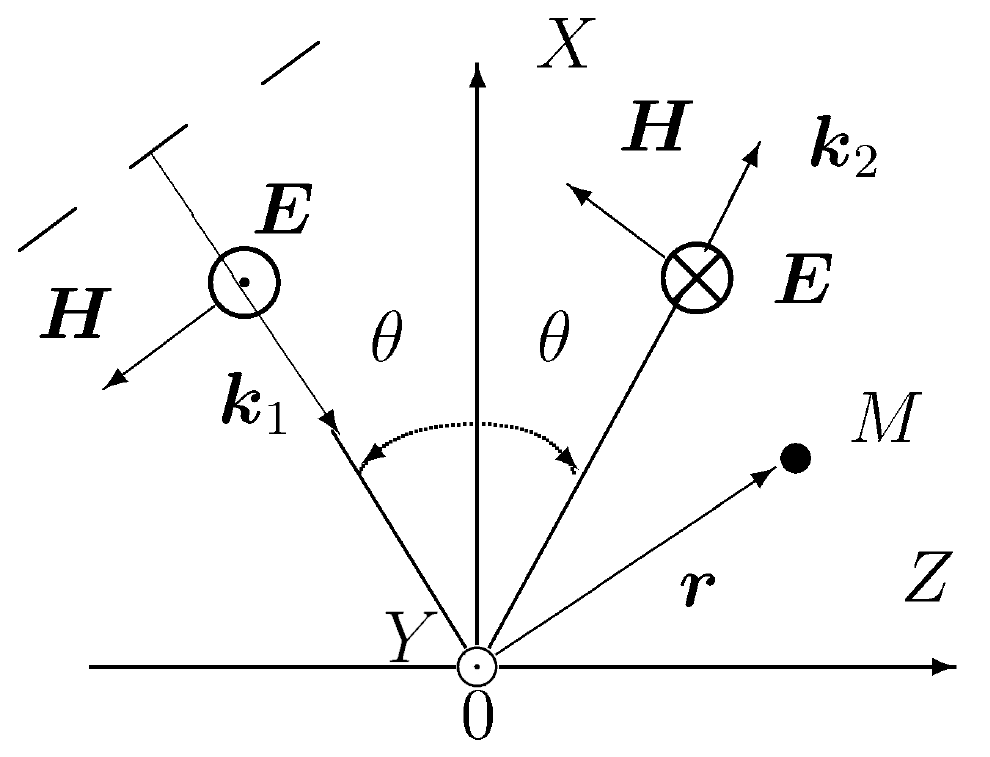
\includegraphics[width=7cm]{1.png}
\caption{Отражение плоской волны от проводящей плоскости}
\end{wrapfigure}
\n
В произвольную точку $M$ приходят две волны: падающая $\bm{E_{\text{пад}}}$ и отражённая $\bm{E_{\text{отр}}}$. При этом
\[ E_{\text{пад}} = E_0 \x \exp(i(\omega t - \bm{k_1 r})), \]
\[ E_{\text{отр}} = - E_0 \x \exp(i(\omega t - \bm{k_2 r})), \]
\n
где $k_1 = k_2 = \omega / c$. Знак <<-->> в отражённой волне связан со сдвигом фаз на $\pi$ при отражении.
\n\n
Суммарное поле в точке $M$ имеет вид
\[E = E_0 \x (e^{(i(\omega t - \bm{k_1 r})} - e^{i(\omega t - \bm{k_2 r})}).\]
\n\n
Подставим $\bm{r} = [x, 0, z]$, $\bm{k_1} = [-k \cos \theta, 0, k \sin \theta]$, $\bm{k_1} = [k \cos \theta, 0, k \sin \theta]$:
\[E = 2iE_0 \sin(kx \cos \theta) \x e^{i\omega (t - z \sin \theta / c)}.\]
\n
Это выражение описывает волну с амплитудой $2iE_0 \sin(kx \cos \theta)$, бегущую в направлении $z$ с фазовой скоростью $\upsilon_{\text{ф}} = c / \sin \theta$. Ясно, что в результате интерференции в пространстве над проводящей поверхностью образуется система стоячих волн. Узлы стоячей волны наблюдаем в точках, где $kx \cos \theta = \pi n$ ($n = 0, 1, 2, ...$), т.е. там, где
\[x = \frac{\pi n}{k \cos \theta}.\]
\n
Таким образом, поверхность нулевого электрического поля - плоскость, параллельная отражающей поверхности. Расположим в этой плоскости вторую проводящую поверхность. Эта поверхность не исказит полученного распределения поля, т.к. на ней удовлетворяются граничные условия $E(t) = 0$. Точно такие же плоскости можно поставить, например, при $y = 0$ и $y = b$.\n\n
%Э.м. поле в волноводе не является чисто поперечным, а имеет продольные составляющие. В нашем случае отлична от нуля продольная составляющая магнитного поля - имеем $H$-волну. Если бы мы взяли другую поляризацию ($H = H_y$), возникла бы $E$-волна.\n\n
Условие распространения волн между параллельными плоскостями, расположенными на расстоянии $a$ друг от друга:
\[cos \theta_n = \frac{\pi n}{ka} = \frac{n \lambda_0}{2a} = \frac{\pi n c}{a \omega} \leq 1,\]
\n
где $\lambda_0$ - длина волны в свободном пространстве. Существует наименьшая критическая частота, при которой волна ещё может проходить через волновод:
\[\omega_{\text{кр}} = \frac{\pi c}{a}.\]
\n
Тогда выражение для фазовой скорости принимает вид:
\[\upsilon_{\text{ф}} = \frac{c}{\sin \theta} = \frac{c}{\sqrt{1 - \cos ^2 \theta}} = \frac{c}{\sqrt{1 - (\omega_{\text{кр}} / \omega)^2}},\]
а волновое число, описывающее распространение волны вдоль волновода, рассчитывается по формуле:
\[k_z = \frac{\omega}{\upsilon_{\text{ф}}} = \frac{\omega}{c} \sqrt{1 - \left (\frac{\omega_{\text{кр}}}{\omega} \right )^2}.\]
\n
Преобразуем это соотношение, связав длины волн в волноводе ($\lambda_{\text{в}}$), в открытом пространстве ($\lambda_0$), и критическую ($\lambda_{\text{кр}}$):
\[\frac{1}{\lambda_{\text{в}}^2} = \frac{1}{\lambda_0^2} - \frac{1}{\lambda_{\text{кр}}^2}.\]
\n
Если в волноводе имеется какое-либо препятствие (в предельном случае волновод закрыт металлической пластиной), то в нём появляется отражённая волна. В результате интерференции образуется стоячая волна:
\[E_{\text{пад}} = E_0 \x \exp(i(\omega t - k_z z)),\]
\[E_{\text{отр}} = \rho E_0 \x \exp(i(\omega t + k_z z + \varphi)),\]
\n где $\rho$ - коэффициент отражения по амплитуде, $\varphi$ - фаза отражённой волны.
Суммарное поле в волноводе равно
\[E(z) = E_{\text{пад}} + E_{\text{отр}} = E_0 e^{-ik_z z} \x (1 + \rho e^{i(2k_z z + \varphi)})e^{i\omega t} = A_0 e^{i \omega t}.\]
\n
%Из этого выражения видно, что в каждом сечении волновода ($z = const$) поле зависит от времени по гармоническому закону, а квадрат амплитуды равен
%\[A_0^2 = E_0^2 \x (1 + \rho^2 + 2 \rho \cos (2k_z z + \varphi)).\]
Максимальное и минимальное значения поля равны соответственно
\[E_{max} = E_0(1 + \rho), \qquad E_{min} = E_0(1 - \rho),\]
\n
а расстояние между соседними узлами (или пучностями) составляет
\[l = \frac{\pi}{k_z} = \frac{\lambda}{2}.\]
\n
Это даёт удобный способ измерения длины волны $\lambda$ в волноводе.
\n\n
Отношение
\[K = \frac{E_{max}}{E_{min}}\]
\n
называется коэффициентом стоячей волны. Через него можно выразить коэффициент отражения по амплитуде:
\[\rho = \frac{E_{max} - E_{min}}{E_{max} + E_{min}} = \frac{K - 1}{K + 1}.\]
\n
\section*{Экспериментальная установка}
\subsection*{Волны в волноводе при частоте выше критической}

\begin{figure}[H]
\centering
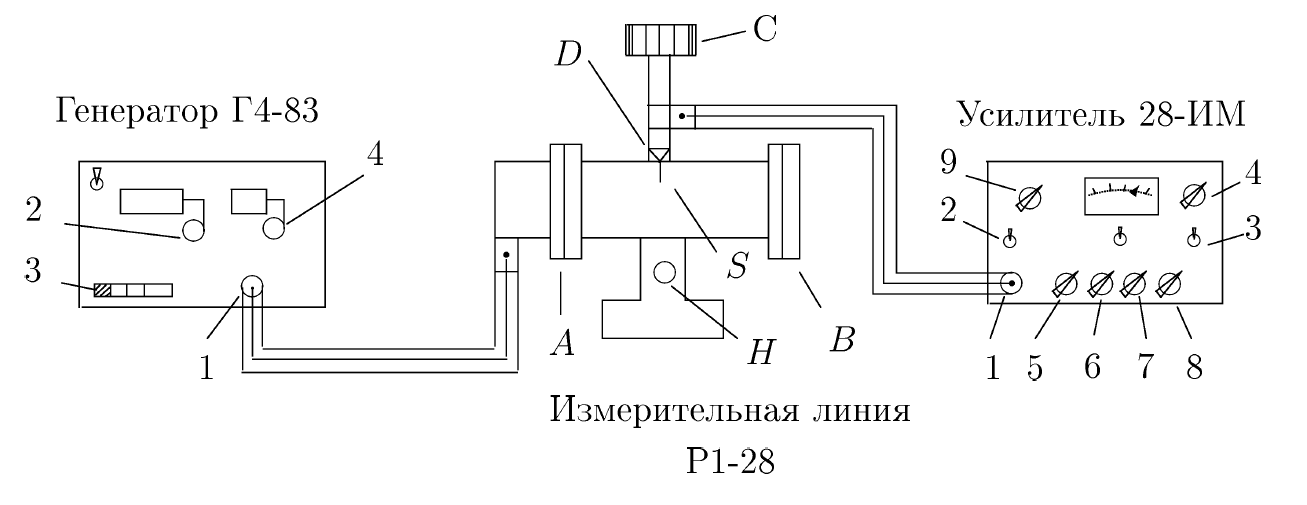
\includegraphics[width=0.8\textwidth]{2.png}
\caption{Схема для исследования структуры волн СВЧ}
\end{figure}

Модулированный сигнал от высокочастотного генератора поступает на вход А измерительной линии, вдоль которой перемещается зонд S. Высокочастотный сигнал с зонда поступает на кристалический детектор D, с его нагрузки (RC-цепочки) снимается огибающая сигнала и подаётся на усилитель низкой частоты. Ручка С предназначена для согласования зонда (как антенны) со входом усилителя. Величина сигнала регистрируется вольтметром, вмонтированным в усилитель.\n\n
Устройство детекторной головки таково, что отклик вольтметра $U$ на величину поля $E$ в волноводе
\[U \sim E^n,\]
где показатель степени $n$ сам зависит от величины сигнала: при малых сигналах детектирование квадратичное, при больших - линейное.

%\subsection*{Б. Волны в волноводе при частоте ниже критической}
%
%\begin{figure}[H]
%\centering
%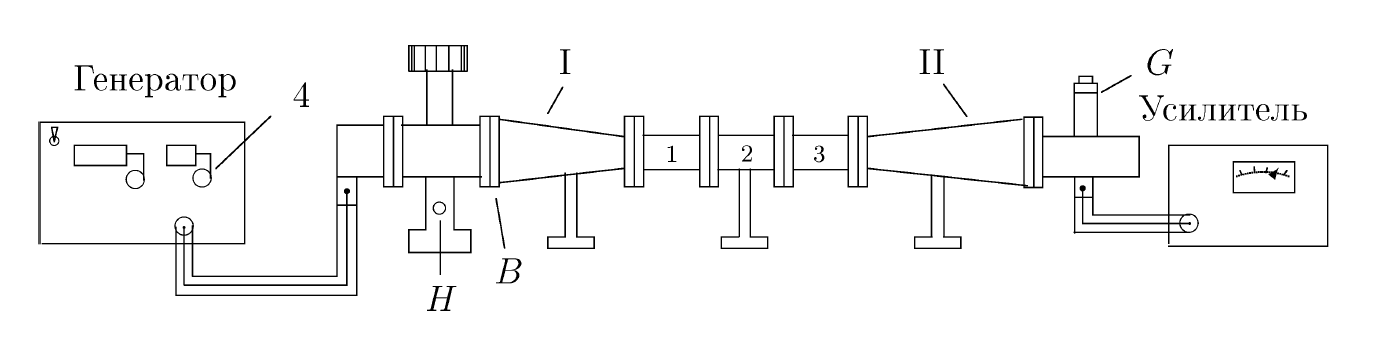
\includegraphics[width=0.8\textwidth]{3.png}
%\caption{Схема для исследования затухания}
%\end{figure}
%
%Используются те же генератор, усилитель, измерительная линия и дополнительный набор волноводов с отдельной детекторной головкой G. В такой системе волны с частотами меньше критической экспоненциально затухают.
%\n\n
%Мощность сигнала на выходе равна
%\[W = W_0 e^{- \alpha z},\]
%\n
%где $W_0$ - мощность входного сигнала, а коэффициент $\alpha z$ измеряется в неперах (1 непер соответствует отношению интенсивностей, равному $e$):
%\[\alpha = 2 i k_z = \frac{2 \omega}{c} \sqrt{\left (\frac{\omega_{\text{кр}}}{\omega} \right )^2 - 1} = \frac{2\pi}{a} \sqrt{1 - \left (\frac{2a}{\lambda_0} \right )^2}, \]
%\n
%где $\lambda_0 = c / \nu = 3.22$ см - длина волны в свободном пространстве, соответствующая рабочей частоте $\nu = 9320$ МГц, $a = 1.6$ см - размер широкой стенки волновода-вставки.

\section*{Обработка результатов измерений}
При подготовке приборов к работе были зафиксированы следующие параметры:
\begin{itemize}
\item Рабочая частота выходного сигнала $\nu = 9320$ МГц
\item Ослабление выходной мощности $\gamma = 20$ дБ
\item Размер стенки волновода $a = 23$ мм
\item Критическая частота $\nu_{\text{кр}} = c / 2a \approx 6500$ МГц
\end{itemize}
\n
В начале волновод с конца был закрыт металлической пластиной. Перемещая зонд, мы настроились на пучность стоячей волны. Была снята зависимость показаний вольтметра $U$ от положения зонда $z$, представленная в таблице и на графике ниже.

\begin{table}[H]
\centering
\begin{tabular}{|l|r|r|r|r|r|r|r|r|r|r|r|r|}
\hline
$z$, мм & 10   & 0    & 4   & 8    & 12   & 16   & 20   & 24   & 28 & 32   & 36   & 40   \\ \hline
$U$, мВ & 2.7 & 3.2 & 0.1 & 1.1 & 5.3 & 8.9 & 6.6 & 1.1 & 0.0  & 2.4 & 7.3 & 8.7 \\ \hline
\end{tabular}
\end{table}

\begin{wrapfigure}{l}{12cm}
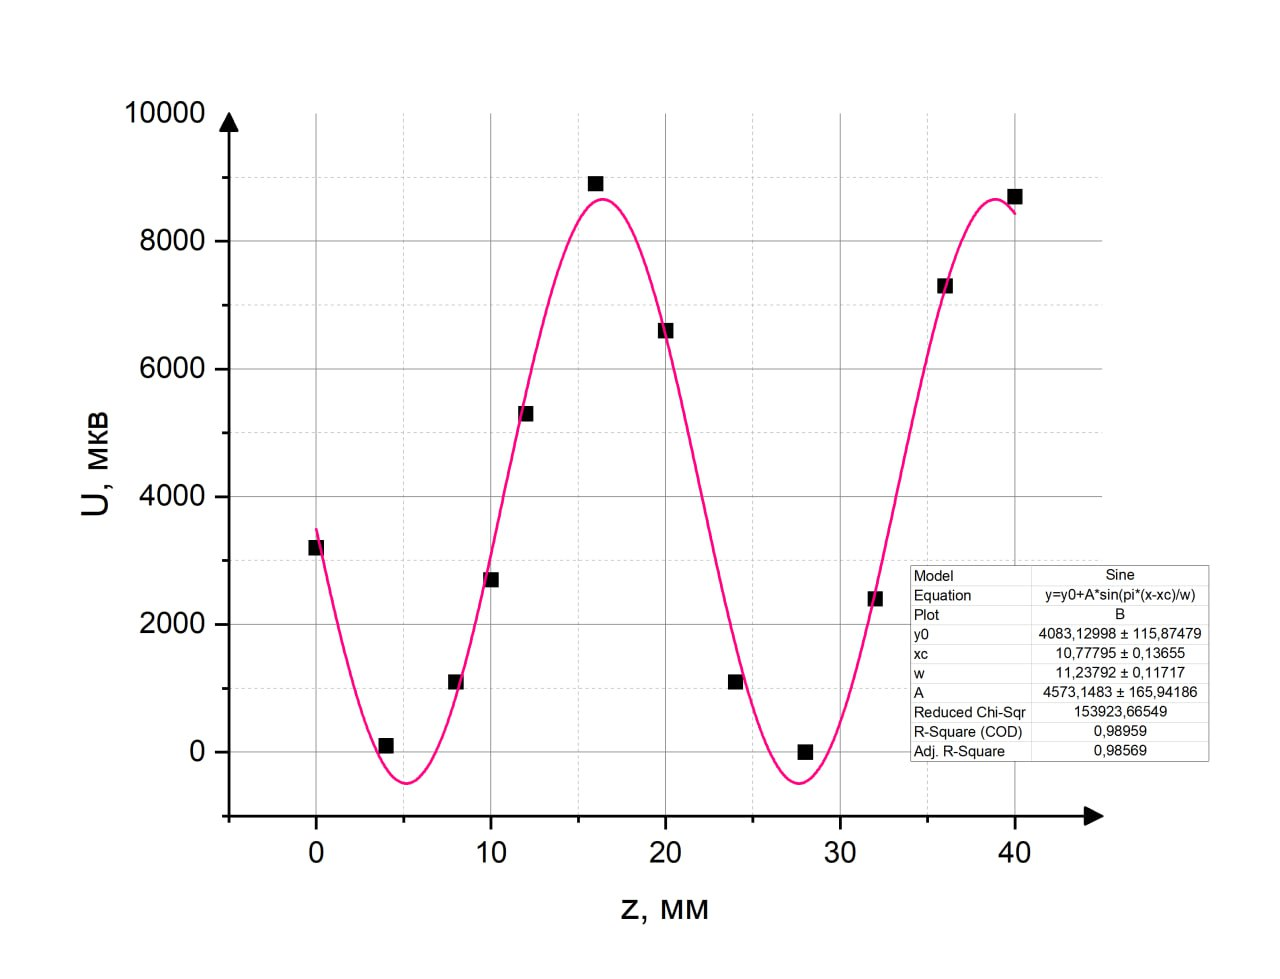
\includegraphics[width=12cm]{plot_1.png}
\caption{Зависимость показаний вольтметра от положения зонда}
\end{wrapfigure}
\n
По графику можно определить длину волны в волноводе:
\n
$\lambda_{\text{в}} \approx 2 \x (28 - 4) \text{ мм} = (48 \pm 4) \text{ мм}.$
\n\n
Рассчитаем $\lambda_{\text{в}}$ теоретически: $\lambda_{\text{кр}} = 2a = 46$ мм, $\lambda_0 = 3.22$ см $\Rightarrow$ $\lambda_{\text{в}} = 45$ мм.
\n\n
Значение, полученное практически, в пределах погрешности совпадает с теоретическим, что говорит об исправности зонда и точной настройке приборов.
\n\n
Длина волны в свободном пространстве $\lambda_{0} = 32.2$ мм меньше критической длины волны $\lambda_{\text{кр}} = 46.0$ мм.
\n\n
Фазовая скорость равна $\upsilon_{\text{ф}} = (42 \pm 5) \x 10^4$ км/c.
\n\n
Групповая скорость равна $\upsilon_{\text{гр}} = \frac{c^2}{\upsilon_{\text{ф}}} = (21 \pm 2) \x 10^4$ км/c.
\n\n
Затем зонд был установлен в узел стоячей волны. Мы сняли зависимость $U$ от координаты зонда $z$ вблизи минимума. Результаты измерений представлены в таблице ниже.

\begin{table}[H]
\centering
\begin{tabular}{|l|r|r|r|r|r|r|r|r|r|}
\hline
$z$, мм & 25.5 & 26.0 & 26.5 & 27.0 & 27.5 & 28.0 & 28.5 & 29.0 & 29.5 \\ \hline
$U$, мкВ & 546  & 312 & 144  & 54 & 12   & 36 & 120  & 246 & 432  \\ \hline
\end{tabular}
\end{table}
\n
По этим данным можно построить график зависимости $\ln U$ от $\ln (\sin (k_z \x \Delta z))$, где $\Delta z$ - это абсолютное смещение от узла. В нашем случае $z_{\text{узла}} = 27.5$ мм.

\begin{wrapfigure}{r}{11cm}
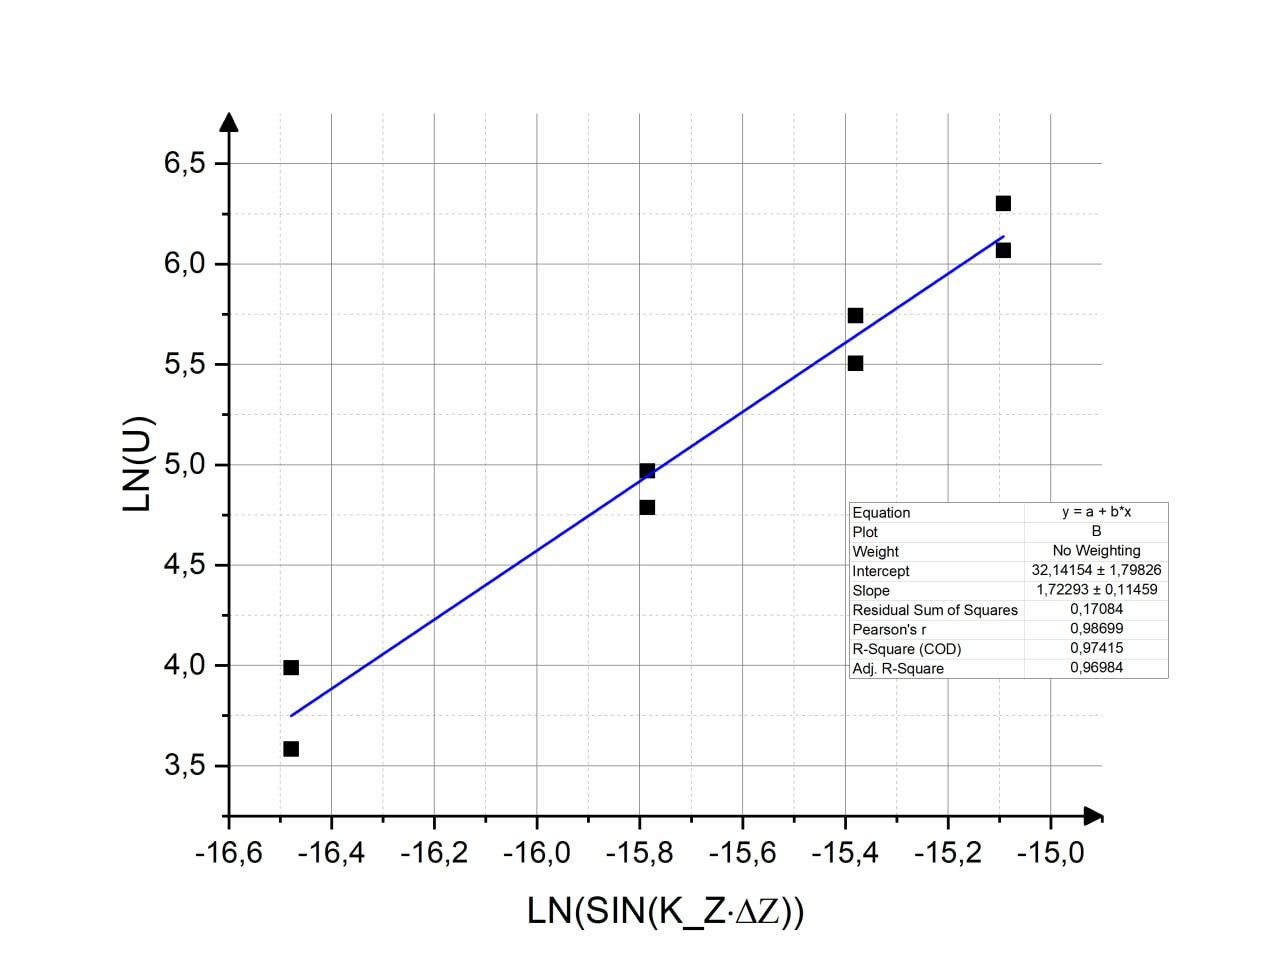
\includegraphics[width=11cm]{plot_2.png}
\caption{График зависимости $\ln U$ от $\ln (\sin (k_z \x \Delta z))$}
\end{wrapfigure}
\n
Видно, что график отражает линейную зависимость. По наклону прямой можно определить характер детектирования: $\tg(\alpha) \approx 1.7 \Rightarrow n = 2$. Получили, что детектирование квадратичное.
\n\n
На следующем шаге работы мы сняли заглушку с фланца измерительной линии. Перемещая зонд, измерили максимальное и минимальное напряжение в волне:
\[U_{max} = 1860 \text{ мкВ}, \qquad U_{min} = 540 \text{ мкВ}.\]
\n
То же самое было проделано с надетым на фланец отрезком с поглощающей нагрузкой:
\[U_{max} = 1110 \text{ мкВ}, \qquad U_{min} = 810 \text{ мкВ}.\]
\n
После этого мы определили коэффициенты отражения (считая детектирование квадратичным) для открытого ($r_1$), закрытого ($r_2$) волновода и волновода с поглощающей нагрузкой ($r_3$):
\[r_1 = (0.55 \pm 0.07), \qquad r_2 = (0.99 \pm 0.12), \qquad r_3 = (0.16 \pm 0.02).\]
\n
При этом $r_2^{\text{теор}} = 1$, $r_3^{\text{теор}} = 0$.
\section*{Заключение}
В закрытом волноводе мы действительно наблюдали стоячие волны. Были рассчитаны длина волны в волноводе $\lambda_{\text{в}} = (48 \pm 4)$ мм (в пределах погрешности сходится с теоретическим предсказанием), фазовая скорость $\upsilon_{\text{ф}} = (42 \pm 5) \x 10^4$ км/с, групповая скорость $\upsilon_{\text{гр}} = (21 \pm 2) \x 10^4$ км/с. Мы определили характер детектирования - квадратичный.
Также были рассчитаны коэффициенты отражения. Объяснить полученные результаты можно следующим образом: когда волновод наглухо закрыт металлической заглушкой, волна практически полностью отражается, при этом $r$ близко к 1: $r_2 = (0.99 \pm 0.12)$; когда на конце волновода находится вещество, поглощающее СВЧ-излучение, коэффициент отражения близок к 0: $r_3 = (0.16 \pm 0.02)$; воздух не препятствует распространению СВЧ-волн, но в воздушной среде излучение становится менее интенсивным: $r_1 = (0.55 \pm 0.07)$.

\section*{Список литературы}
\begin{enumerate}
\item \textit{Сивухин Д.В.} Общий курс физики. -- Т.III. Электричество. -- М.: Наука, 1983. \textsection 84.
\item \textit{Фейнмановские} лекции по физике. Т. 6. Электродинамика. -- М.: Наука, 1966. Гл. 24.
\item \textit{Кингсеп А.С., Локшин Г.Р., Ольхов О.А.} Основы Физики. Т.1. Механика, электричество и магнетизм, колебания и волны, волновая оптика. -- М.: ФИЗМАТЛИТ, 2001. Ч. II, Гл. 8, \textsection 8.4; Ч.III, Гл. 6, \textsection 6.7.
\end{enumerate}

\section*{Работу провели}
Киркича Андрей, Клименко Виталий, Гришин Михаил

\end{document}